
分光光度法是用于确定药物分子的简单,快速和准确的方法。该方法基于两种试剂之间形成复合物。许多复合物是有色的,并在可见光区域有吸收。因此可以用分光光度法测定它们。

抗组胺药物\textbf{D}作为给电子基团,与$\pi$-受体\textbf{S}复合。所得的复合物在最大吸收(460 nm)处记录的吸光度与药物浓度线性相关,具有良好的相关系数。
$$
\begin{aligned}
\mathrm D+\mathrm S\rightleftharpoons\mathrm {DS}\\
K=\frac{[\mathrm{DS}]}{[\mathrm D][\mathrm S]}\\
\end{aligned}
$$
其中\([\mathrm{DS}]\),\([\mathrm D]\)与\([\mathrm S]\)分别代表\textbf{DS}复合物,\textbf{D}与\textbf{S}的平衡浓度。
\[
c_{\mathrm D}=[\mathrm D]+[\mathrm {DS}]
\] 
其中\(c_{\mathrm D}\)是药物的总浓度。

只有所形成的\textbf{DS}络合物可以吸收光的波长下,以下表达式成立:

 \[
A=\varepsilon_{\mathrm{DS}}l[\mathrm{DS}]
\] 
其中\(l\)是吸收池长度。

可以使用Benesi--Hildebrand方程来计算络合物的结合平衡常数,该方程取决于实验条件,其中一种组分应大量过量,以使其浓度不会随复合物的形成而改变。

\[
\frac{c_{\mathrm D}}{A_{\mathrm{DS}}}=\frac{1}{\varepsilon_{\mathrm{DS}}}+\frac{1}{\varepsilon_{\mathrm{DS}}K}\times\frac{1}{c_{\mathrm S}}
\]
其中\(c_{\mathrm S}\)与\(c_{\mathrm D}\)是\textbf{S}与\textbf{D}的总浓度。\(A_{\mathrm{DS}}\)是复合物的吸光度,\(\varepsilon_{\mathrm{DS}}\)是复合物的摩尔吸光系数,\(K\)是平衡常数。

\begin{figure}[h]
	\centering
	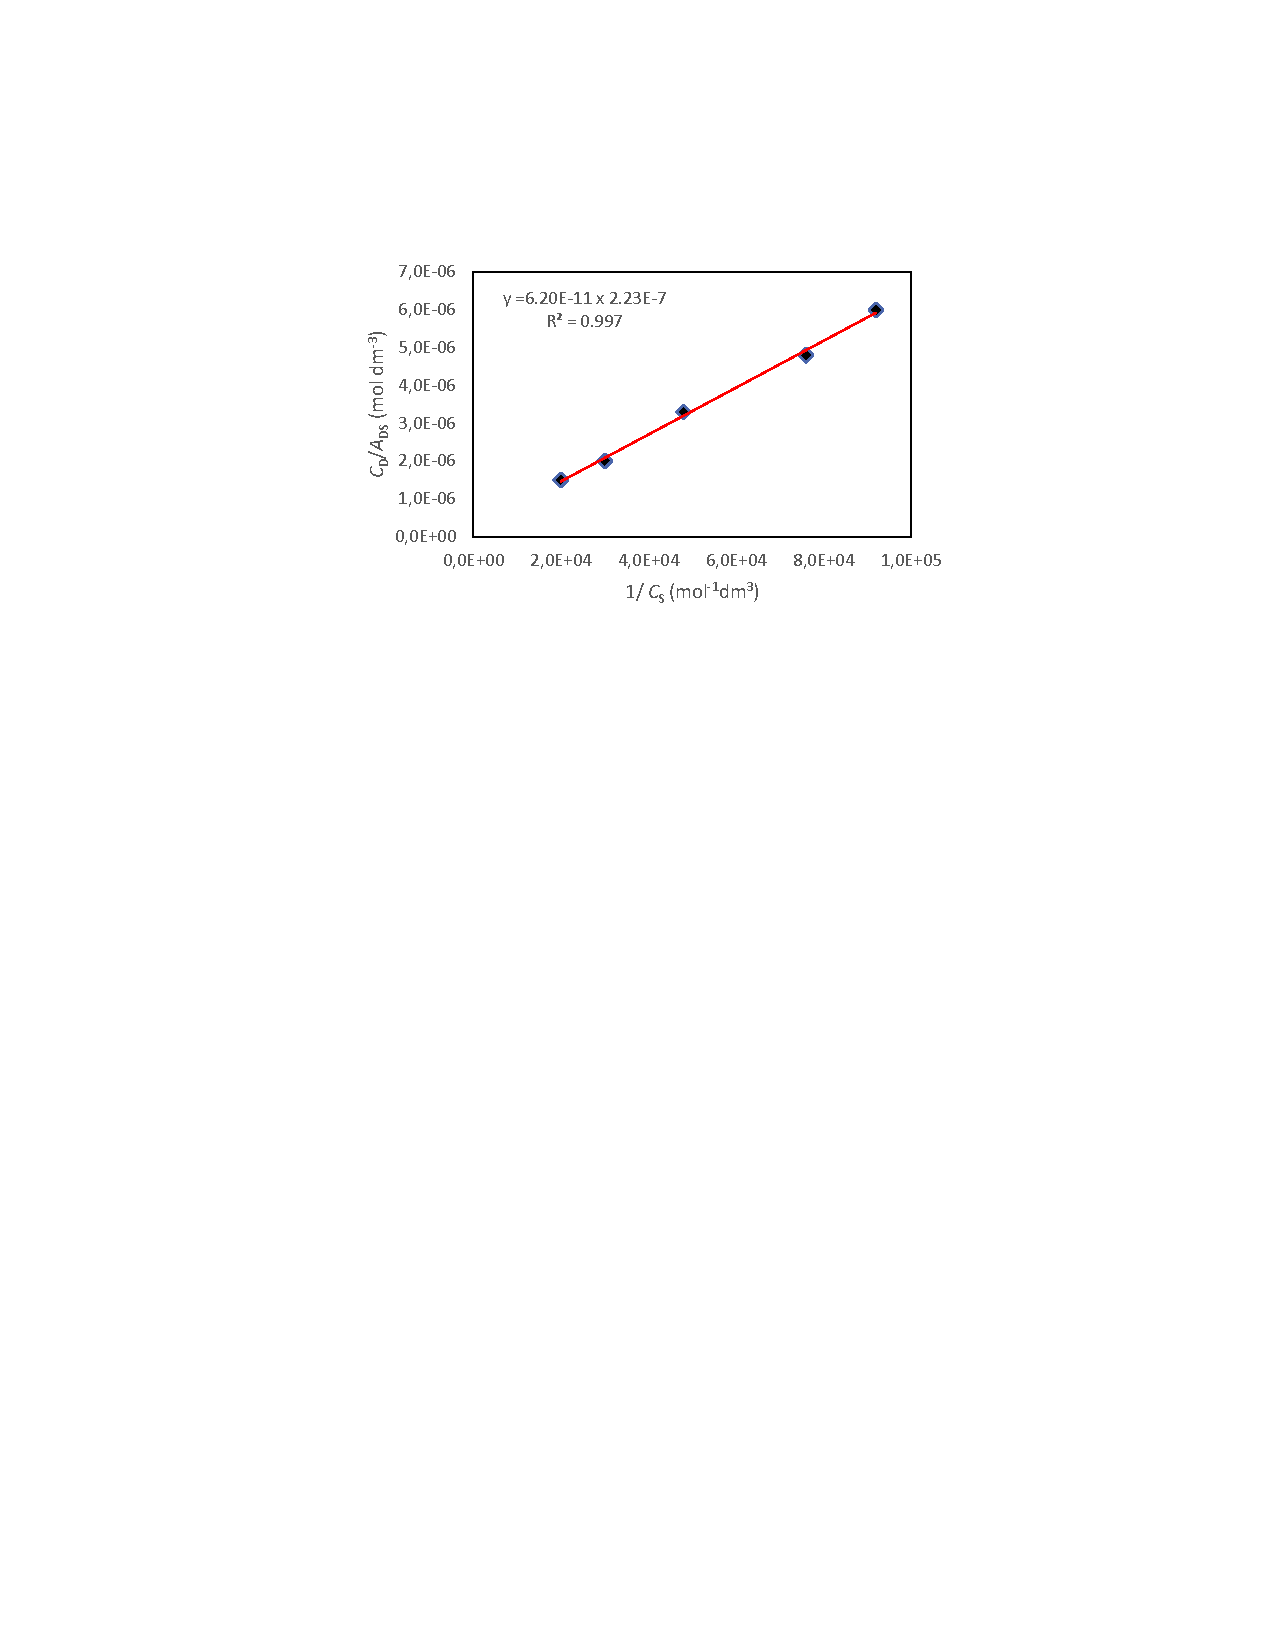
\includegraphics[width=12cm]{./pic/t25-1.pdf}
\end{figure}

\noindent\textbf{25.1.} 考虑在25
°C下记录的Benesi--Hildebrand图,给出复合物生成的平衡常数和复合物的摩尔吸光系数。


\noindent\textbf{25.2.}
\textbf{D}与\textbf{S}的起始浓度是9×10\textsuperscript{−5} mol
L\textsuperscript{−1},计算平衡时复合物形成的百分数。\textbf{D}与\textbf{S}在复合的时候比例为1:1。

\noindent\textbf{25.3.} 计算25 °C下的\(\Delta_rG^\ominus\),单位为kJ
mol\textsuperscript{−1}。

通过改变温度(25、45和60 °C)研究\textbf{D}与\textbf{S}的络合动力学。该表给出了在不同温度下的络合速率常数。

\begin{longtable}[]{@{}llll@{}}
	\toprule
	$T$ (°C) &25&45&60 \tabularnewline
	$k$ (min\textsuperscript{--1}) & 0.0200 &0.0504&0.0944\tabularnewline
	\bottomrule
\end{longtable}

\noindent\textbf{25.4.} 计算活化能\(E_a\)。

\noindent\textbf{25.5.}
已知\(k_{\mathrm{TST}}=\frac{k_{\mathrm BT}}{h}e^{-\frac{\Delta G^\ddag}{RT}}\),计算25 °C下的活化焓\(\Delta H^\ddag\),活化熵\(\Delta S^\ddag\)以及活化自由能\(\Delta G^\ddag\)。
(译注:原文为自由活化焓\(\Delta G^\ddag\))
